\chapter{\uppercase {Validation}}
\label{sec:validations}

\section{\aetherflow Validation}


We use the \aetherflow implementation described in \ref{sec:impl} to
evaluate the performance and demonstrate the viability of the \aetherflow
approach. 
Our results demonstrate that \aetherflow framework allows SDN 
applications to efficiently and dynamically configure wireless
networks without loss of performance. 

%In particular, we extend its
%capability by adding event report and statistics methods. We add a socket on
%both hostapd and ofsoftswitch13 sides for their inter process communication.
%When an event occurs, hostapd sends a notification to ofsoftswitch13 daemon to
%notify, and the daemon will then send to the controller with the corresponding
%experimenter message we defined above to notify the controller, if the event is
%of interest to the controller. When the controller needs to query the statistics
%of mobile stations on an access point, it sends the query to ofsoftswitch13
%first. ofsoftswitch13 forwards the request to hostapd. hostapd invokes API of
%driver to obtain the statistics and sends back the statistics to ofsoftswitch13,
%which then proxy the information back to controller.

%Supports of \aetherflow configurations also needs to be added. Authentication
%procedure of hostapd needs to be modified to support the authentication
%profile/group model. In particular, the original hostapd only supports `one-
%shot' authentication, i.e. only authenticate each mobile station once during
%the association procedure. Our model requires multiple attempts of
%authentication based on different profiles. The other configurations, including
%radio interface configuration and access point configurations, are implemented
%in a different way. Parameters in these configurations are all configurable
%with OpenWRT's UCI system. Therefore when such configuration requests are sent
%by the controller, the switch will handle them by invoking corresponding
%OpenWRT APIs to reconfigure the parameters.

\subsection{Experiment Setup}
Our experiment uses a simple network topology, shown in Figure~\ref{fig:topology}. 
It consists of two access points (AP1, AP2), a Layer 2 switch, a wireline 
traffic generator and a wireless 802.11 mobile station (STA).  We use an OpenFlow enabled
Layer 2 switch and  \aetherflow enabled APs as described in Section~\ref{sec:impl}. The mobile station has a single WiFi radio
interface. 

\begin{figure}
\centering
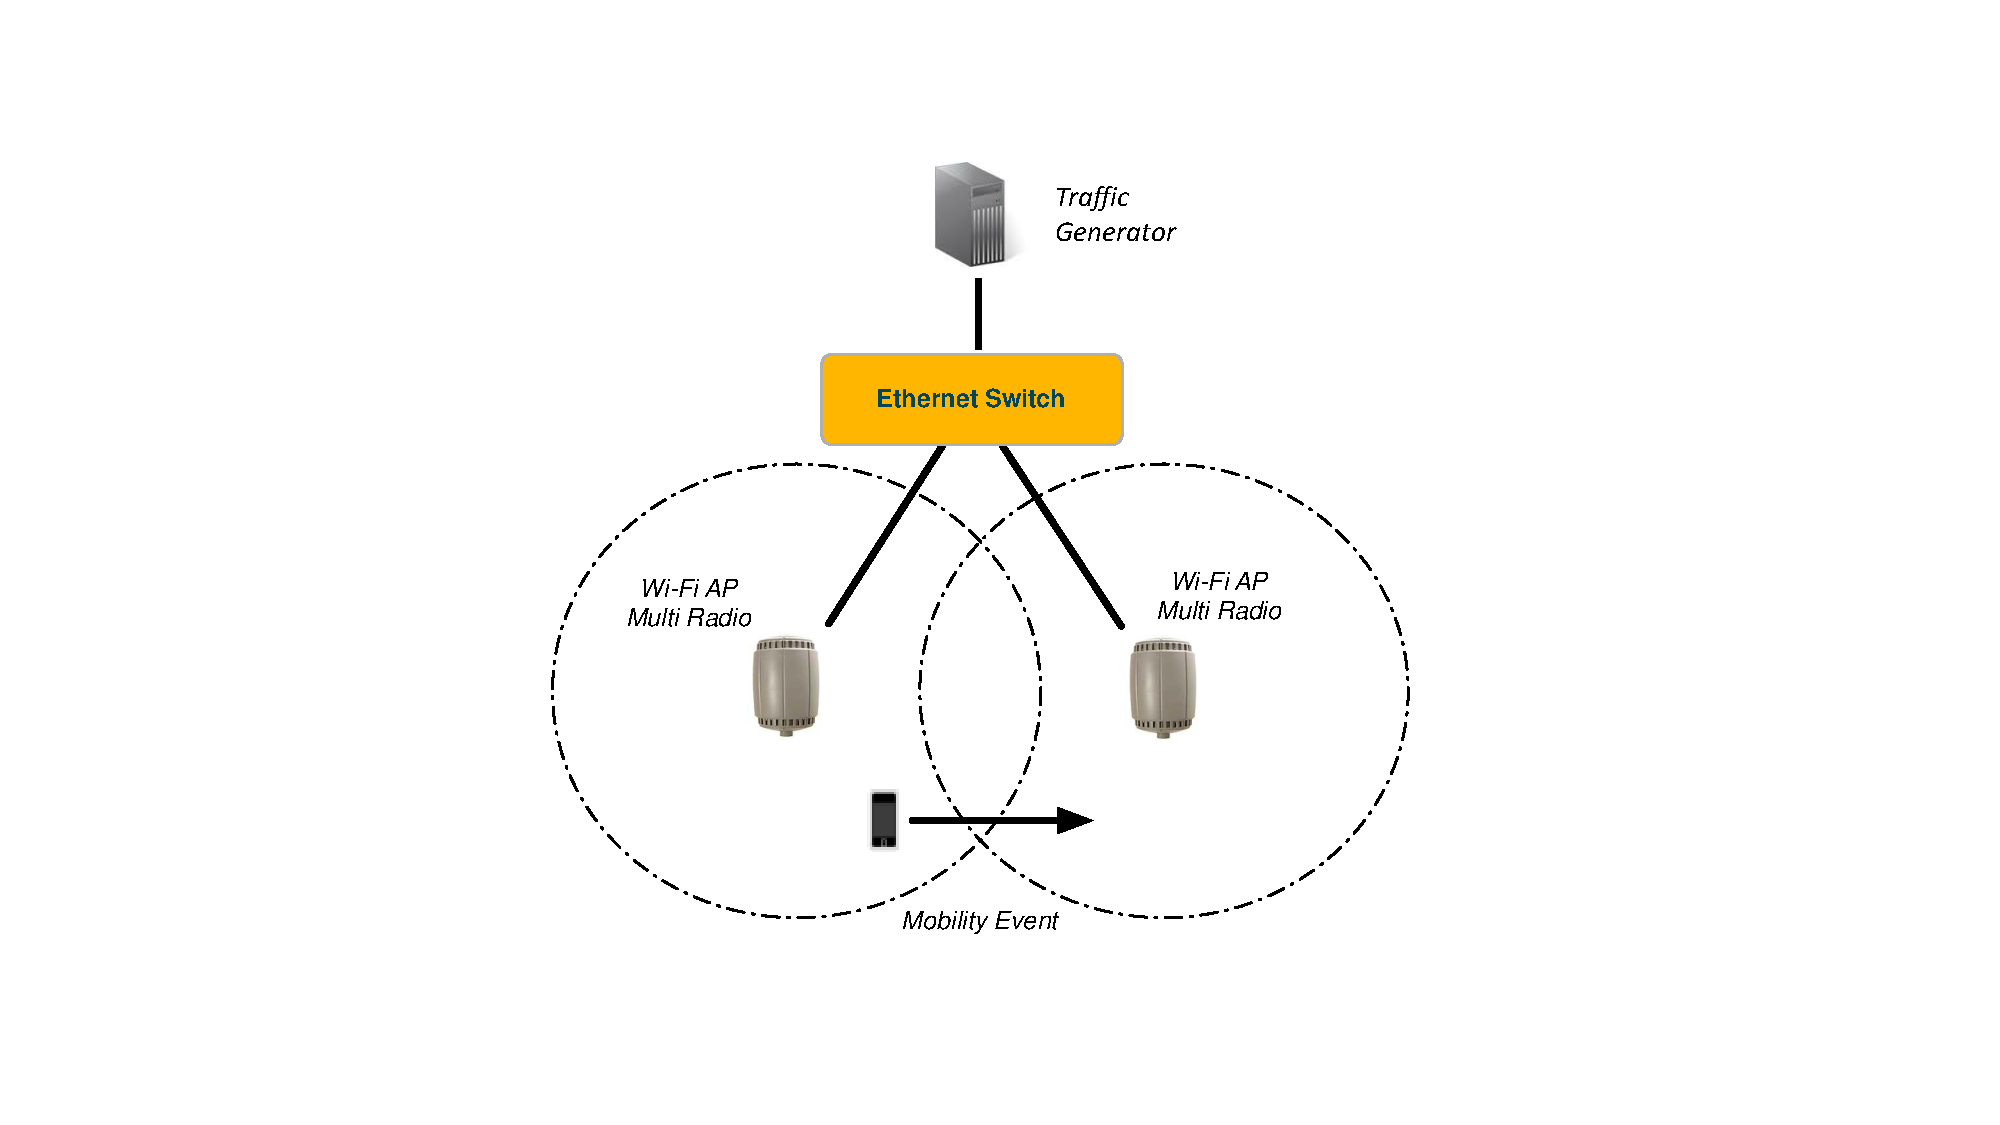
\includegraphics[width=1.0\textwidth]{figures/topology}
\caption[\aetherflow Experiment network topology]{Experiment network topology\protect\footnotemark}
\label{fig:topology}
\end{figure}

In our experiment, both APs and the traffic generator are connected to the switch
through  Ethernet. All the three boxes are connected to an OpenFlow
controller through a separate control plane subnet that is not displayed in the
figure.  The two APs are located at a certain distance and have overlapping coverage areas.  Both APs are configured with
the same SSID and use open authentication. 

\subsection{Layer 2 Handoff Application}
Our Layer 2 handoff application accords with what we described in
Section~\ref{sec:application}. The investigation of good
predictors and predictive models for handoff is beyond the scope of this paper.
In our implementation, the controller application always predicts that the
handoff of STA from AP1 to AP2 will occur seven seconds after the experiment starts.
The time period is selected solely for the purpose of this experiment and
does not apply for general cases. 
 
\footnotetext{Courtesy: flowgrammable.org}
After seven seconds, the controller starts to multicast packets going to STA to both
AP1 and AP2 by sending FlowMod messages to both APs and the switch. After STA
associates with AP2, the controller configures the switch to stop multicasting
and forward packets to only AP2. If the predicted handoff did not happen 15
seconds after the prediction, the controller reverts the multicast and forwards
packets to only AP1.



\subsection{Experiment Procedure and Results}
In each round of experiment, the mobile station is initially associated with AP1. Both the traffic generator
and the mobile station are assigned static IP addresses within the same subnet. Before the experiment
starts, a UDP \texttt{iperf} session with bandwidth of 9Mbps is initiated from
the traffic generator to STA.  After experiment starts, STA moves from coverage
of AP1 to coverage of AP2, which forces the client to handoff from AP1 to AP2.
We move STA in a controlled manner such that the handoff happens at seven seconds
after the experiment starts. This time is selected such that the handoff happens
almost immediately after the controller application initiates multicasting.  Throughput
and packet loss rate during each round of test is measured by iperf with an
interval of 0.5s. In each round of experiment, one of the following
configurations is used:
\begin{itemize}
\item {\bf Bridge configuration} uses neither OpenFlow nor \aetherflow. Instead,
the Layer 2 switch and the two APs use the Linux built-in learning bridge to
forward packets. This is the traditional way of configuring a Layer 2 network
with two access points and one switch. 
\item {\bf \aetherflow configuration with prediction} enables \aetherflow on the APs and the
switch, and the handoff is managed by the Layer 2 handoff application (described
above) running on the \aetherflow controller using the Ryu controller framework.  
\item {\bf \aetherflow configuration without prediction} enables \aetherflow on the APs and the
switch, and the handoff is managed by a similar Layer 2 handoff application as given above without enabling prediction.  
\end{itemize}

%\begin{figure*}
%\centering
%  \begin{subfigure}[a]{\textwidth}
%        \centering
%      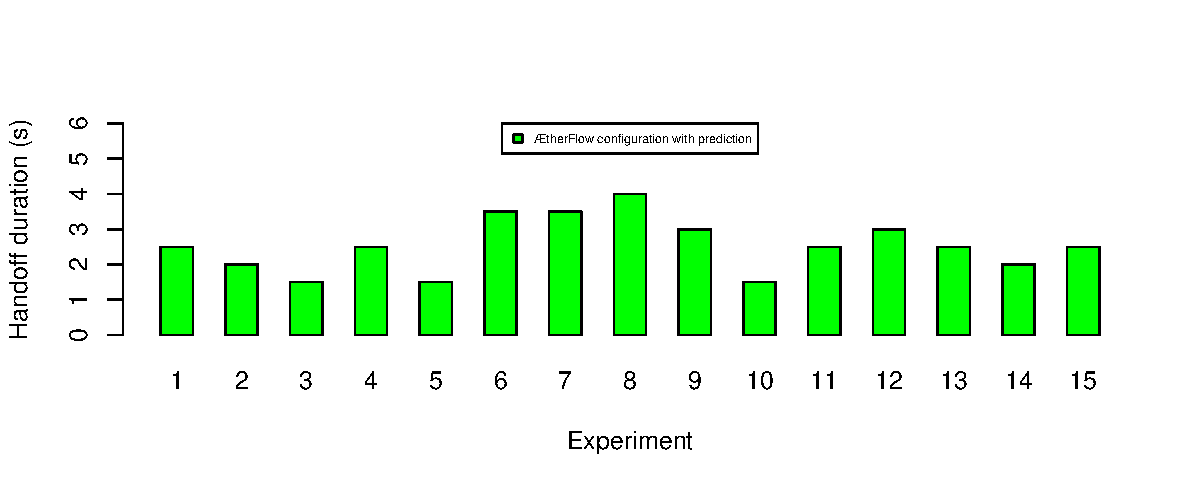
\includegraphics[width=1\textwidth]{figures/predduration.pdf}
%      \caption{Handoff duration for \aetherflow configuration with prediction}
%      \label{fig:pred}
%  \end{subfigure}

%  \begin{subfigure}[b]{\textwidth}
%        \centering
%      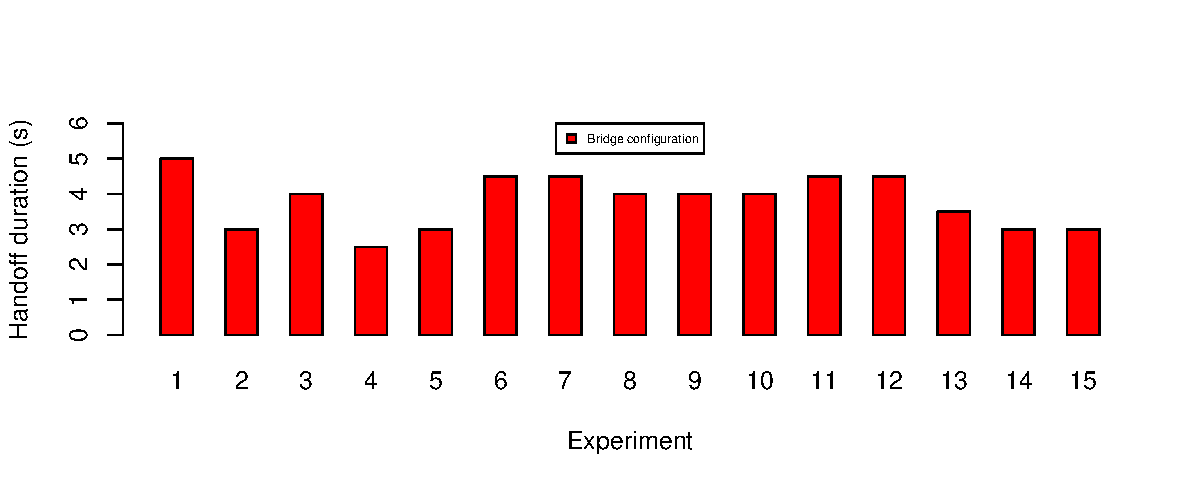
\includegraphics[width=1\textwidth]{figures/bridgeduration.pdf}
%      \caption{Handoff duration for bridge configuration}
%      \label{fig:bridge}
%  \end{subfigure}

%  \begin{subfigure}[c]{\textwidth}
%  \centering
%      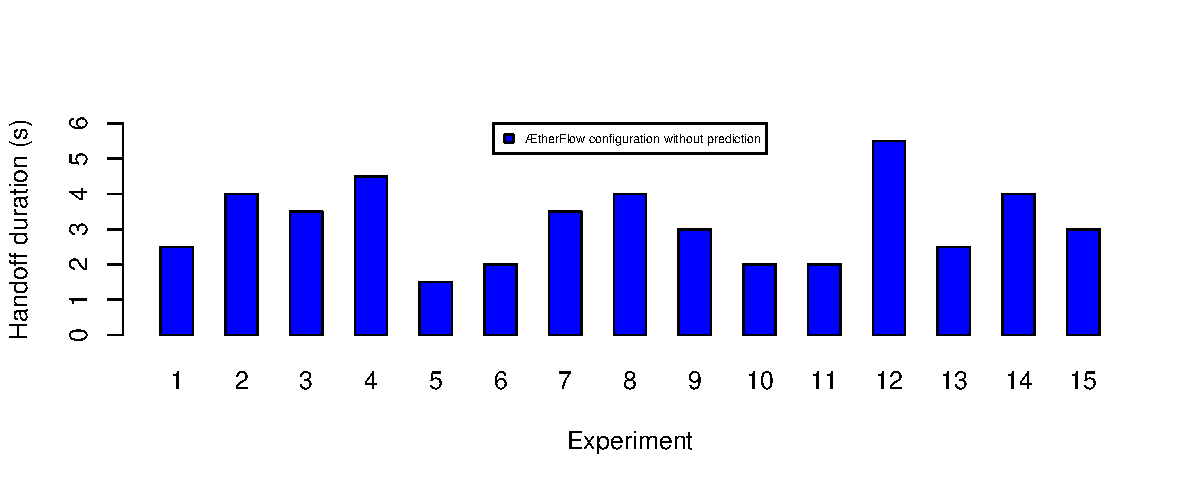
\includegraphics[width=1\textwidth]{figures/simpleduration.pdf}
%      \caption{Handoff duration for \aetherflow configuration without prediction}
%      \label{fig:simple}
%  \end{subfigure}%
%  \caption{Comparision of handoff duration for each experiment type}
%  \label{fig:duration}
%\end{figure*}

Fifteen rounds of experiments are conducted on each of the three configurations given
above. In a single round of experiment, the mobile station is considered to be
in handoff process during an interval after time $t$ = 7s if its average
throughput during the interval is less than 8 Mbps. By this criteria we can
determine the handoff duration of STA in each round of experiment. Our results, depicted  in Figure~\ref{fig:confidence}, indicate that the average handoff
duration of \aetherflow configuration with ~prediction across the fifteen rounds of experiments is
\textbf{2.53}s, which is lower than that of bridge configuration \textbf{3.8}s and \aetherflow configration without prediction \textbf{3.17}s.

We compare the traffic throughput and packet loss rate of the experiments
which have median handoff duration in \aetherflow with prediction and bridge configurations (experiment 3 for
bridge configuration and experiment 4 for \aetherflow configuration). 
The plots are shown in Figures~\ref{fig:throughput} and \ref{fig:loss}. 
These plots demonstrate that in terms of both throughput and loss rate, the \aetherflow
configuration recovers from handoff faster than the bridge configuration. 

\begin{figure}
\centering
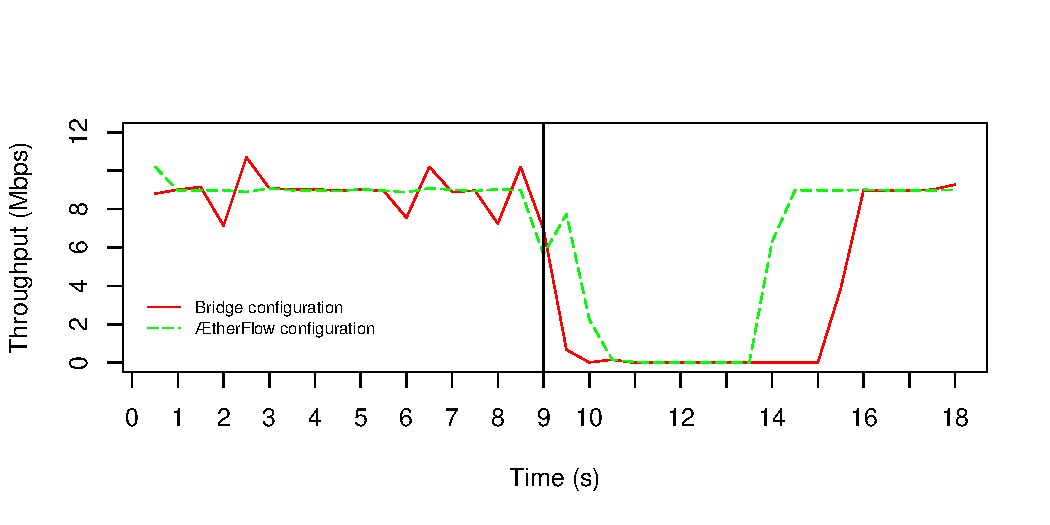
\includegraphics[width=.8\textwidth]{figures/throughput}
\caption{Comparison of throughput for \aetherflow with prediction and the baseline configuration.} % The throughput of
% \aetherflow configuration recovers from handoff in $5.5$ seconds, comparing to
% $7$ seconds in the bridge configuration.} % The total throughput of \aetherflow
% configuration during the handoff ($9$s to $16$s) is $24.5$M while that of the bridge
% configuration is $5.8$M.}
\label{fig:throughput}
\end{figure}

\begin{figure}
\centering
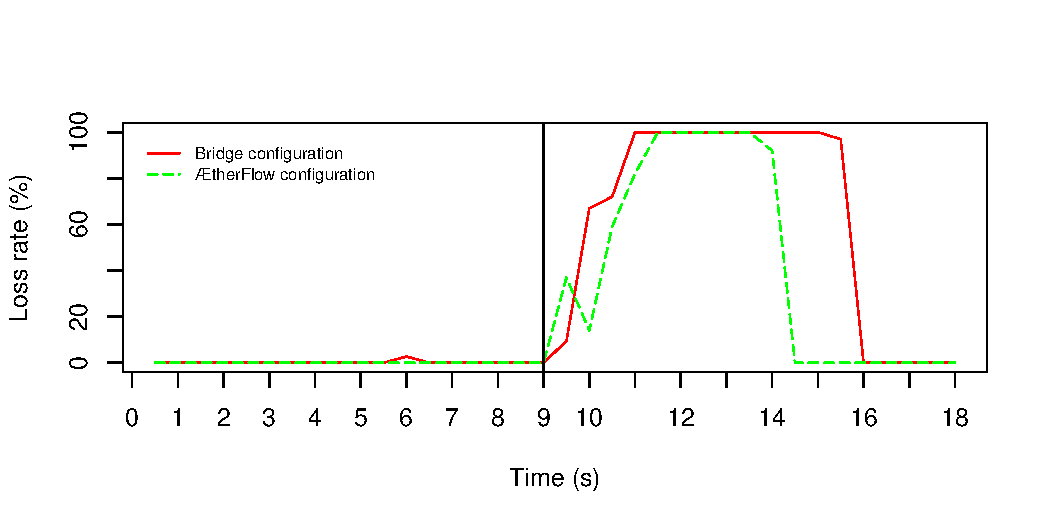
\includegraphics[width=.8\textwidth]{figures/loss}
\caption{Comparison of packet loss rate for \aetherflow with prediction and the baseline configuration.} % The packet loss
% of \aetherflow configuration recovers from handoff in $5.5$ seconds, comparing
% to $7$ seconds in the bridge configuration.}
\label{fig:loss}
\end{figure}

\begin{figure}
\centering
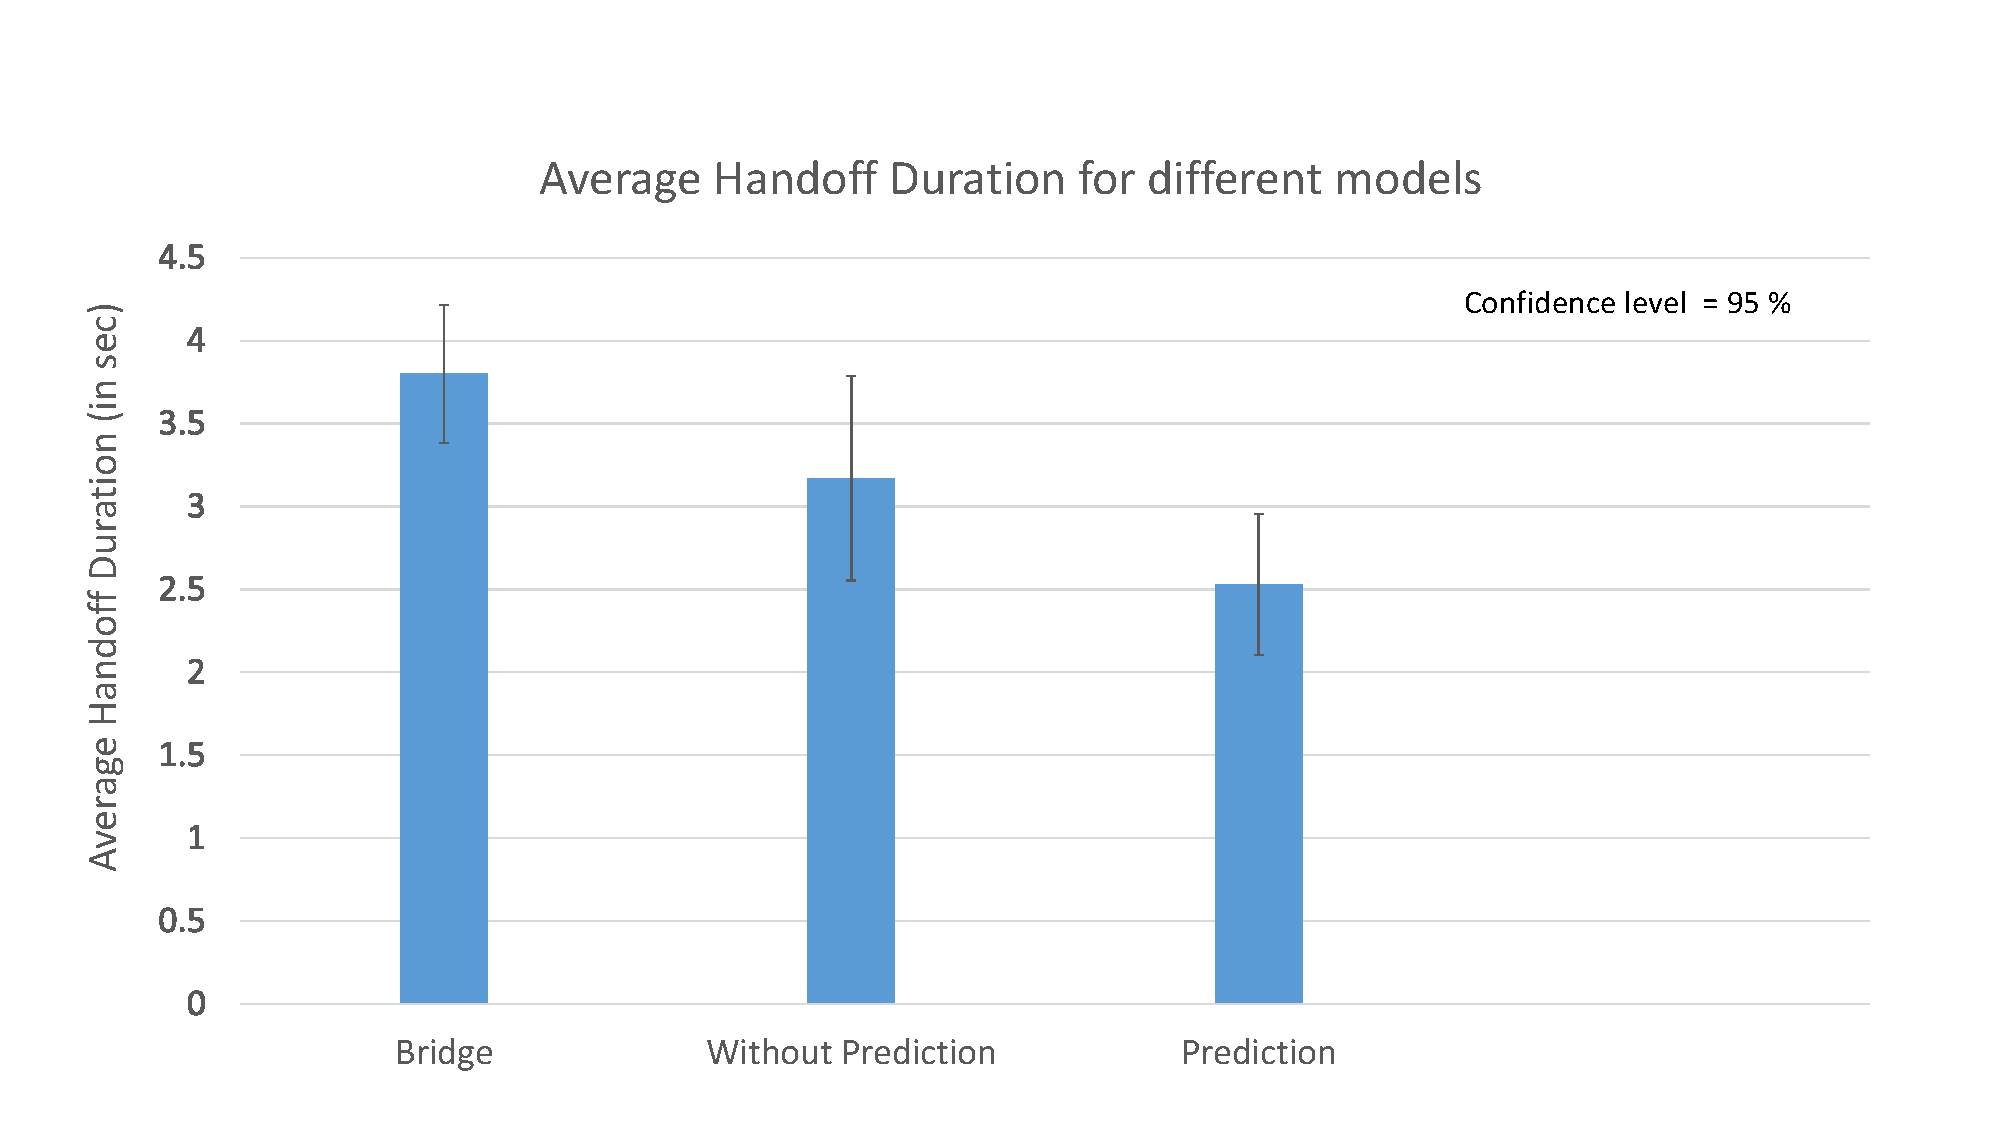
\includegraphics[width=.8\textwidth]{figures/confidence}
\caption{Comparison of average handoff duration for different models with standard error} 
\label{fig:confidence}
\end{figure}

The experiment results show that even with the overhead induced by SDN data plane processing, the performance of Layer~2 handoff application based
on \aetherflow is better that of Linux kernel bridge configuration. % It shows
% that even with the overhead induced by SDN data plane processing, the
% performance of \aetherflow is comparable to that of the traditional configuration. % The results suffice
% for our proof-of-concept demonstration of the \aetherflow framework.



\section{\crossflow Validation}


We use the \crossflow implementation described in \ref{sec:evaluation} to provide a proof-of-concept validation of our design. We demonstrate the viability of \crossflow which  allows SDN applications to change the radio physical properties of wireless radio upon various qualifying parameters like channel conditions. 


\begin{figure*}
\centering
  \begin{subfigure}[b]{\textwidth}
        \centering
      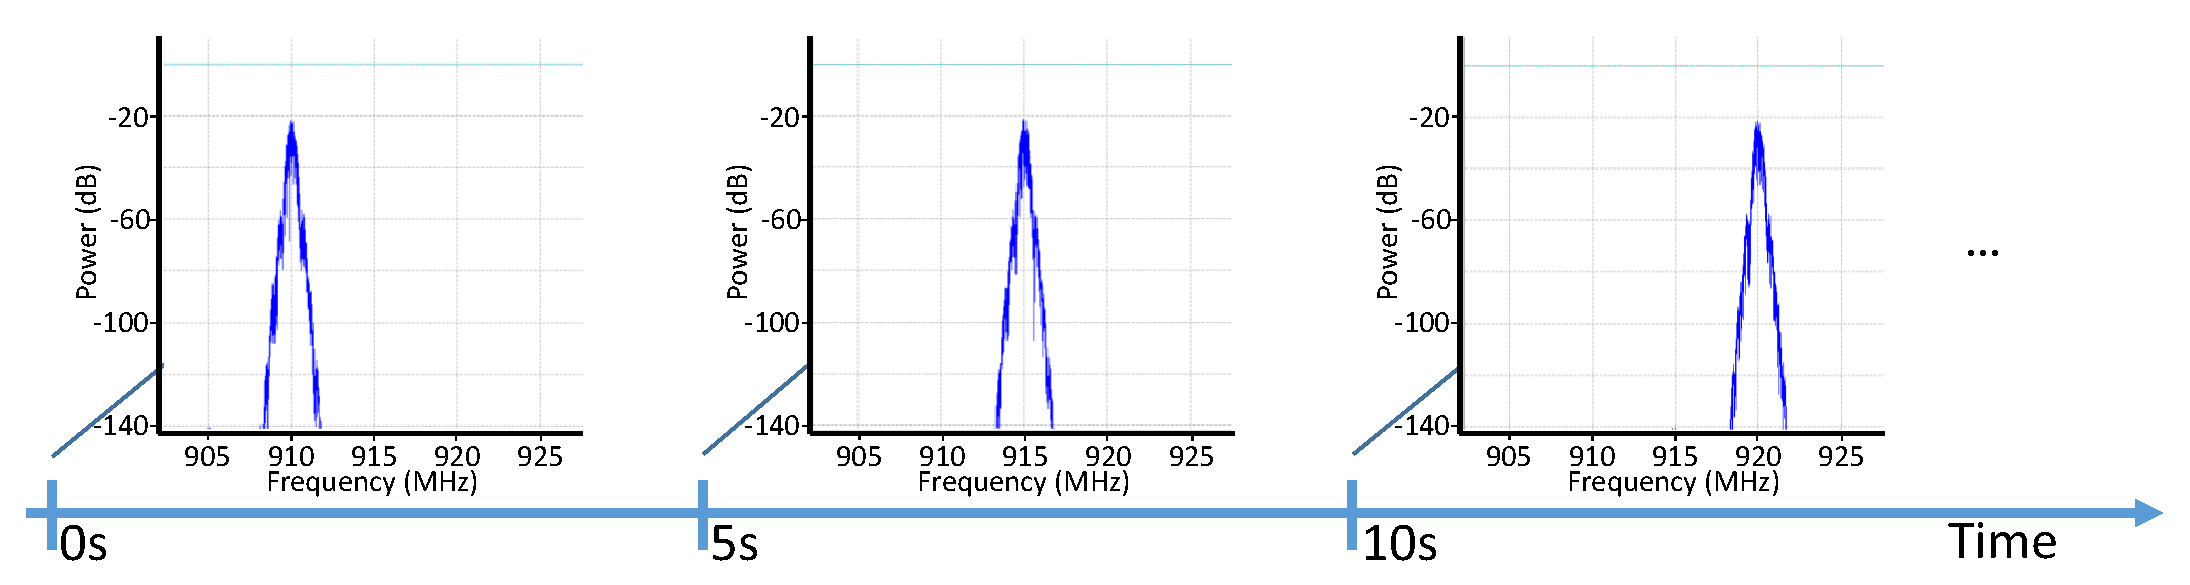
\includegraphics[width=1\textwidth]{figures/Freq.pdf}
      \caption{Spectral output for \emph{frequency hopping} application. The frequency changes every 5 seconds keeping BPSK as a fixed modulation scheme.}
      \label{fig:freq}
  \end{subfigure}

  \begin{subfigure}[a]{\textwidth}
  \centering
      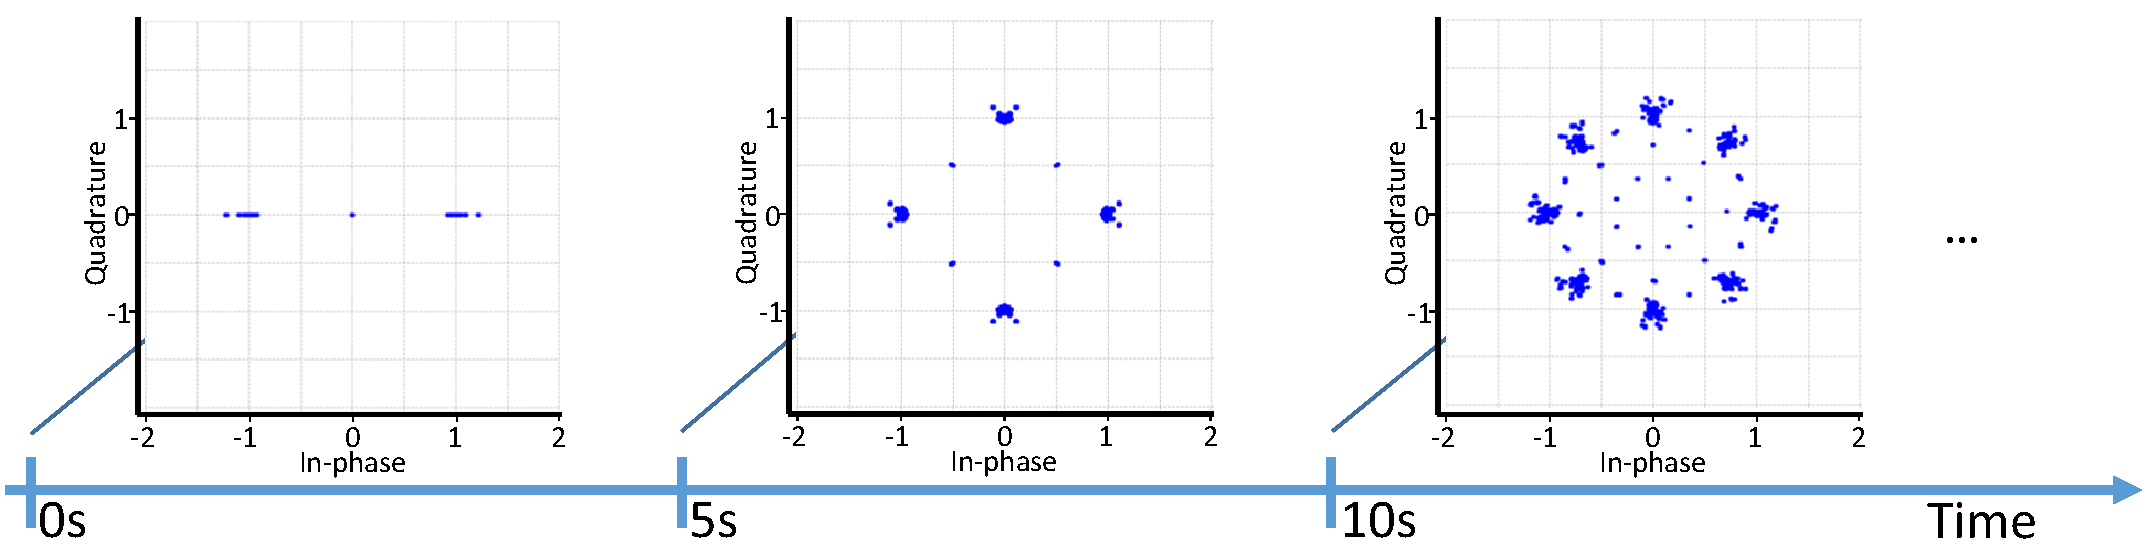
\includegraphics[width=1\textwidth]{figures/Mod.pdf}
      \caption{Constellation output for \emph{adaptive modulation} application. The modulation scheme changes every 5 seconds keeping a fixed frequency of 910 MHz.}
      \label{fig:mod}
  \end{subfigure}%
  \caption{Experimentation results for \emph{frequency hopping} and \emph{adaptive modulation}}
\end{figure*}


\subsection{Frequency Hopping Application Implementation}

In this implementation,  the controller simply issues \emph{GNU-CONFIG-FREQ} command with desired frequency and pushes this configuration to the device. The \texttt{ofsoftswitch} receives this command and forwards it to the GNU Radio domain. The centralized \texttt{\crossflow Hub} inside the GNU Radio domain processes this request and issues appropriate commands to the  USRP Controller, which ultimately signals the USRP block to tune into the requested frequency. Figure~\ref{fig:freq} shows the experimental results where the sequence of changing frequencies is 910, 915 and 920 MHz and is changed every 5 seconds. For this application, we use a fixed BPSK modulation scheme.


\subsection{Adaptive Modulation  Application Implementation}

Similar to the \emph{frequency hopping} application, the controller issues the \emph{GNU-CONFIG-MOD} command with the appropriate modulation scheme (BPSK, QPSK, or 8PSK) and forwards the request to the device. The request ultimately reaches the Mod Controller, which is a multiplexer block that selects the requested modulation scheme. Figure~\ref{fig:mod} shows the results for changing the modulation scheme between BPSK, QPSK and 8PSK every 5 seconds, keeping a fixed carrier frequency of 910 MHz.
